\section{问题求解}

\subsection{问题一的建模与求解}
首先需要对玻璃表面风化情况与玻璃类型,纹饰和颜色的差异性进行分析,并结合玻璃的类型分析化学成分含量的变化规律以及预测风化前的化学成分含量,共需解决三个小问题,问题一建模分析流程图如下图\ref{p-1}所示。
\begin{figure}[!htbp]
	\centering
	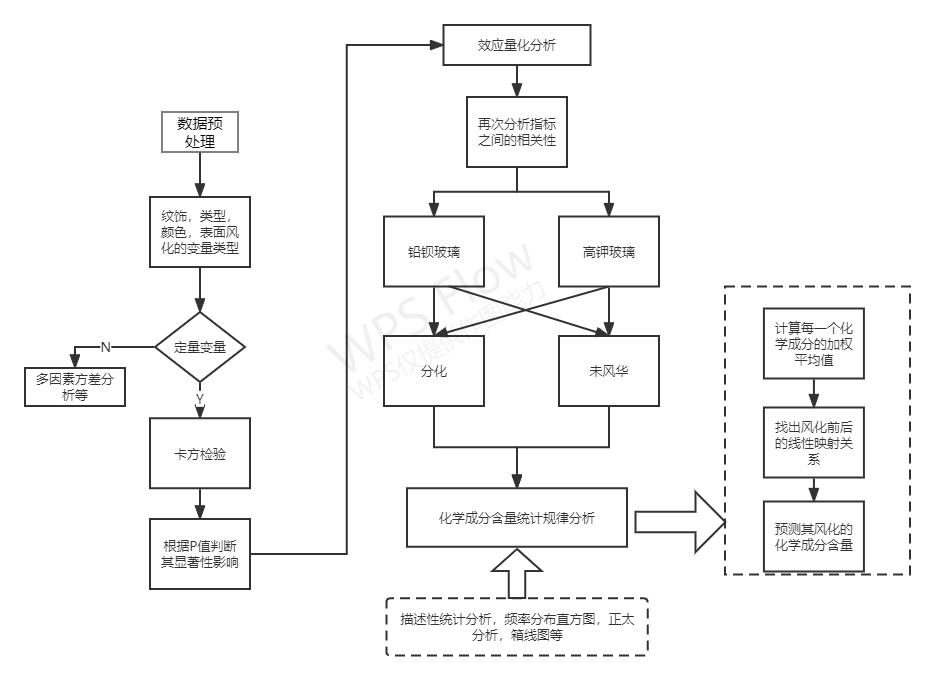
\includegraphics[width=0.6\textwidth]{组织结构图.png}
	\setlength{\abovecaptionskip}{3pt}%caption与表格之间的距离
	\caption{组织结构图}
	\label{p-1}
\end{figure}

\subsubsection{数据预处理}
\begin{enumerate}
	\item 首先进行数据预处理工作,根据题目要求:将成分比例累加和介于85\%~105\%之间的数据视为有效数据。
	\item 附件表单1中颜色列中的数据中,我们发现有四个空值,这里直接删去包含缺失值的样本数据。	
\end{enumerate}

\subsection{独热编码}
独热编码(One-Hot Encoding),又称之为一位有效编码,具体是使用N个寄存器对应N个状态,并且相应状态都有它独立的寄存器位,并且在任意时候,其中只有一位有效。即,只有一位是1,其余都是零值。独热编码 是利用0和1表示一些参数,使用N位状态寄存器来对N个状态进行编码。

通过分析数据,发现玻璃类型、纹饰、颜色变量都与表面是否风化具有一定的相关性。因此通过玻璃类型与表面分化、纹饰与表面风化、颜色与表面分化两两进行比较分析,得出spearman相关系数和复相关系数数据,发现spearman相关系数精确度较高,因此使用spearman相关系数方法来分析此问题,热力图如图\ref{p-16}所示:
\begin{figure}[!htbp]
	\centering
	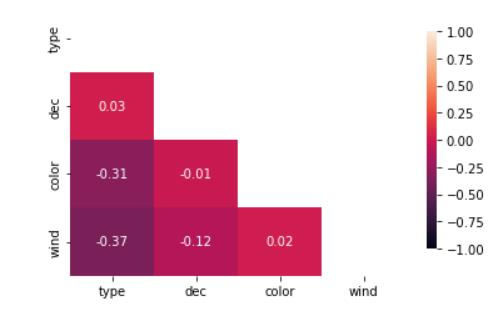
\includegraphics[width=0.7\textwidth]{复相关热力图系数.png}
	\setlength{\abovecaptionskip}{3pt}%caption与表格之间的距离
	\caption{复相关热力图系数}
	\label{p-16}
\end{figure}


\begin{figure}[h]
	\centering
	\begin{minipage}[b]{0.3\linewidth}
		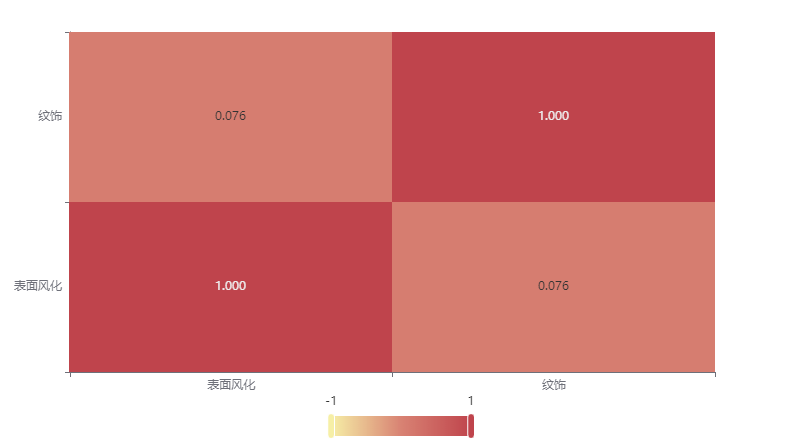
\includegraphics[width=1\textwidth]{s1.png}
	\end{minipage}
	\begin{minipage}[b]{0.3\linewidth}
		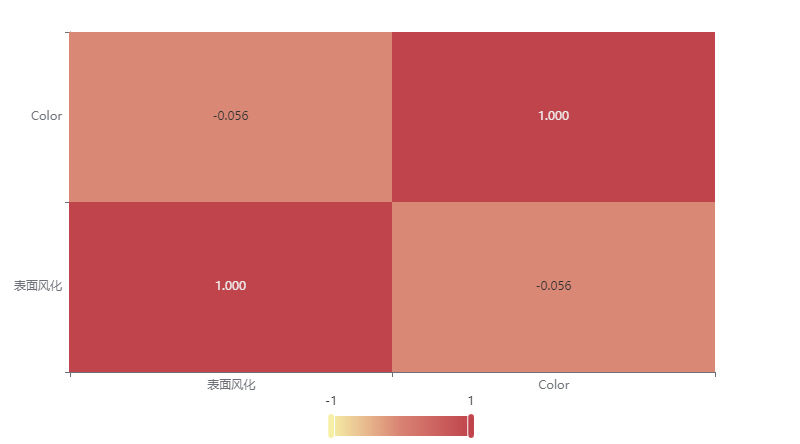
\includegraphics[width=1\textwidth]{s2.png}
	\end{minipage}
	\begin{minipage}[b]{0.3\linewidth}
		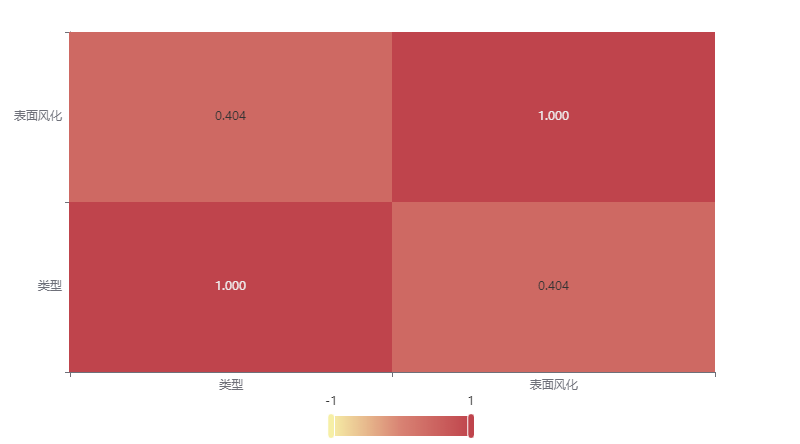
\includegraphics[width=1\textwidth]{s3.png}
	\end{minipage}
	\setlength{\abovecaptionskip}{3pt}%caption与表格之间的距离
	\caption{spearmand系数对比图}
\end{figure}

\subsubsection{针对表面风化情况做卡方检验}
首先通过Python代码将附件表单一和表单二中的数据进行合并,方便接下来的统计,通过观察数据发现纹饰、类型、颜色、表面风化均为定类变量,针对多组定类变量之间的差异性分析我们可以采用卡方检验。

变量X:表面风化;变量Y:纹饰,类型,颜色,使用SPSSPRO软件进行交互分析,得出如下图\ref{p-2}所示的卡方检验表。

\begin{figure}[!htbp]
	\centering
	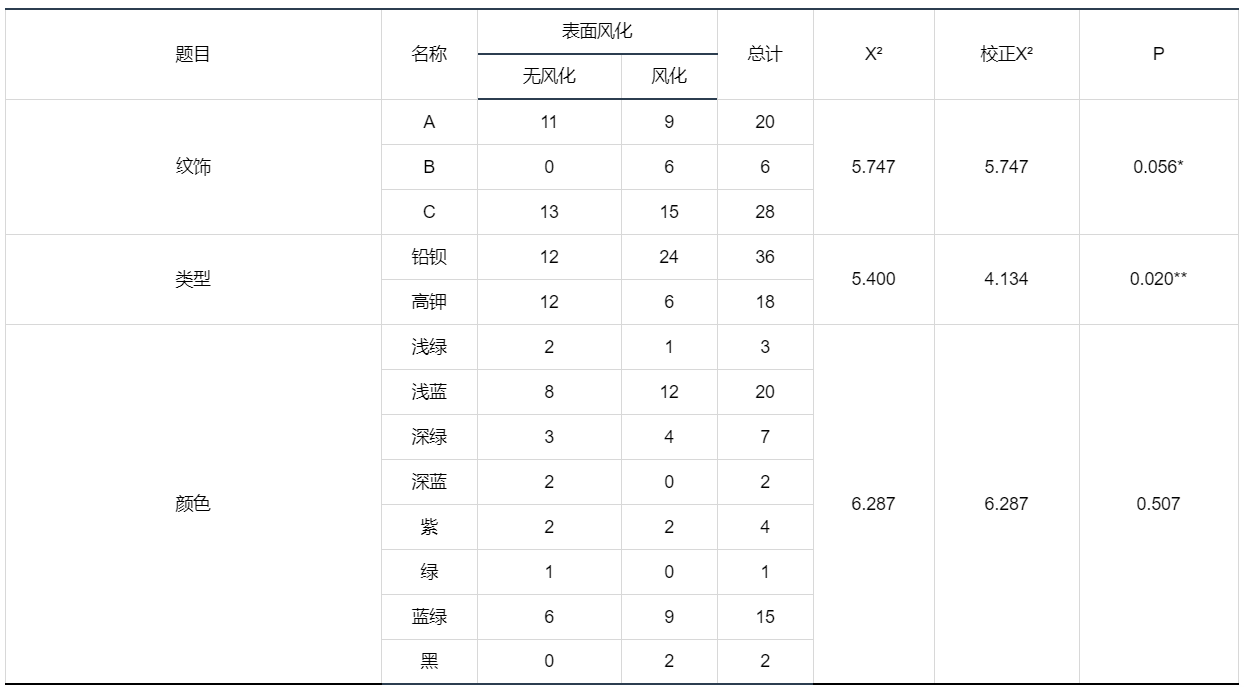
\includegraphics[width=1\textwidth]{卡方检验-类型-颜色-表面风化.png}
	\setlength{\abovecaptionskip}{3pt}%caption与表格之间的距离
	\caption{类型-颜色-表面风化卡方检验表}
	\label{p-2}
\end{figure}

图表说明:
上表展示了模型检验的结果,包括数据的频数、频数百分比、卡方值、显著性P值。
\begin{enumerate}
	\item 分析模型是否呈现出显著性(P值小于0.05或0.01);
	\item 若呈现显著性,拒绝原假设,则说明各样本之间存在显著性差异。具体根据类别的差异百分比进行描述。反之数据不存在显著性差异。
\end{enumerate}


\begin{figure}[h]
	\centering
	\begin{minipage}[b]{0.45\linewidth}
		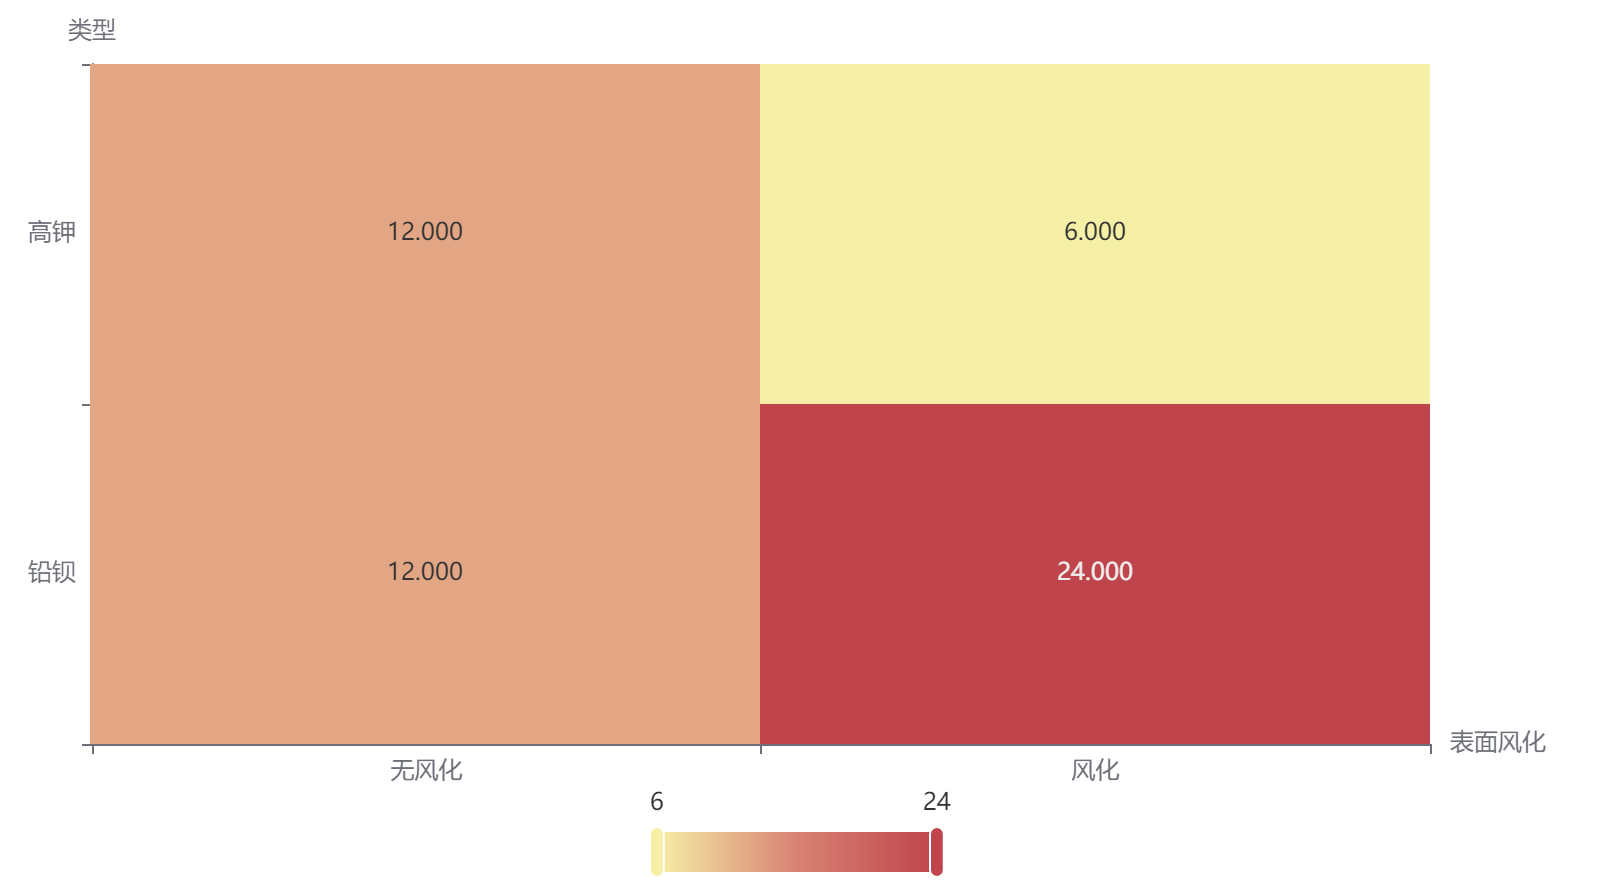
\includegraphics[width=1\textwidth]{表面风化-类型热力图.png}
		\setlength{\abovecaptionskip}{3pt}%caption与表格之间的距离
		\caption{表面风化-类型热力图}
		\label{p-3}
	\end{minipage}
	\begin{minipage}[b]{0.45\linewidth}
		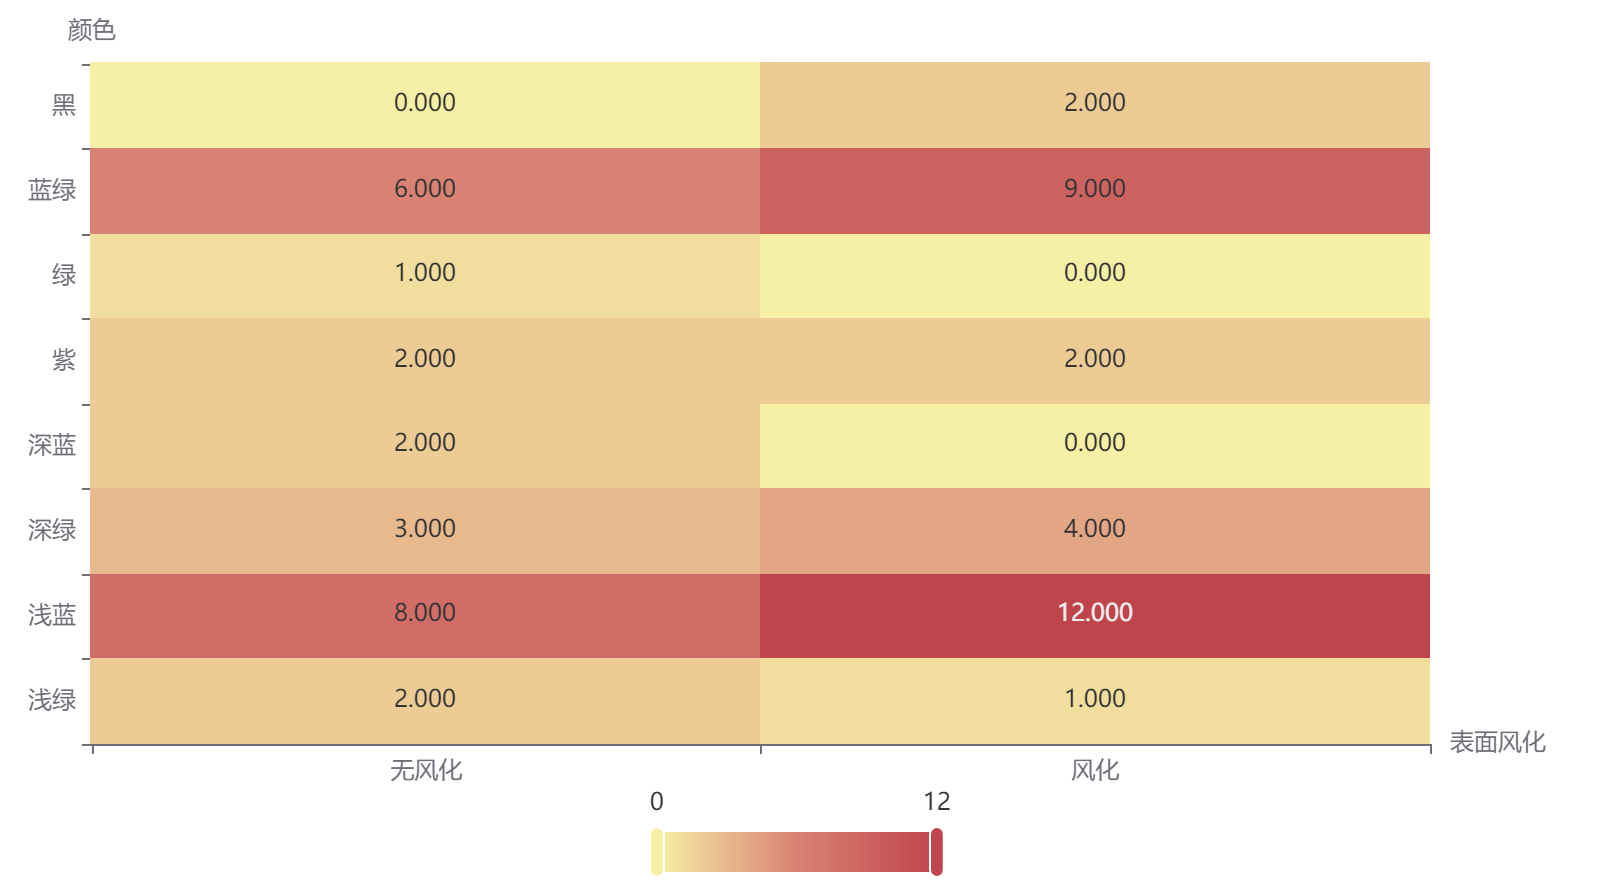
\includegraphics[width=1\textwidth]{表面风化-颜色热力图.png}
		\setlength{\abovecaptionskip}{3pt}%caption与表格之间的距离
		\caption{表面风化-颜色热力图}
		\label{p-4}
	\end{minipage}
\end{figure}

在此基础上进行效应量化分析,包括phi、Crammer's V、列联系数、lambda ,用于分析表面风化与其余三个指标的相关程度,量化分析指标解释如下:
\begin{enumerate}
	\item phi系数: phi相关系数的大小,表示两样本之间的关联程度。当phi系数小于0.3时,表示相关较弱;当phi系数大于0.6时,表示相关较强
	\item Cramer's V: 与phi系数作用相似,但Cramer's V系数的作用范围较广。e3)列联系数:简称C系数。
	\item lambda:用于反应自变量对因变量的预测效果
\end{enumerate}

使用SPSSPRO进行操作,得出结果如下表\ref{t-2}所示。
\begin{table}[h]
	\centering
	\setlength{\abovecaptionskip}{3pt}%caption与表格之间的距离
	\caption{表面风化效应量化分析}
	\vspace{1pt}
	\label{t-2}
	\resizebox{\textwidth}{!}{
		\begin{tabular}{ccccc}
			\toprule[1.5pt]
			\makebox[0.18\textwidth][c]{字段名/分析项} & \makebox[0.18\textwidth][c]{Phi} 
			& \makebox[0.18\textwidth][c]{Crammer's} & \makebox[0.18\textwidth][c]{列联系数}
			& \makebox[0.18\textwidth][c]{lambda} \\ 
			\midrule
			纹饰&	0.326&	0.326&	0.310&	0.000\\
			类型&	0.316&	0.316&	0.302&	0.000\\
			颜色&	0.341&	0.341&	0.323&	0.000\\
			\bottomrule[1.5pt]
	\end{tabular}}
\end{table}

效应量化分析的结果显示,分析项:纹饰 Cramer’s V值为0.326,因此纹饰和表面风化的差异程度为中等程度差异;类型 Cramer’s V值为0.316,因此类型和表面风化的差异程度为中等程度差异;颜色 Cramer’s V值为0.341,因此颜色和表面风化的差异程度为中等程度差异。


\subsubsection{不同类型玻璃表面有无风化化学成分统计规律}
首先使用SPSSPRO软件针对描述性铅钡和高钾两种玻璃风化前后化学成分含量统计分析,结果如下表\ref{t-3}所示:

\begin{table}[h]
	\centering
	\setlength{\abovecaptionskip}{3pt}%caption与表格之间的距离
	\caption{高钾玻璃表面风化效应量化分析}
	\vspace{1pt}
	\label{t-3}
	\resizebox{\textwidth}{!}{
		\begin{tabular}{cccccccccccc}
			\toprule[1.5pt]
			\makebox[0.04\textwidth][c]{变量名} & \makebox[0.06\textwidth][c]{风化情况} 
			& \makebox[0.06\textwidth][c]{样本量} 
			& \makebox[0.05\textwidth][c]{最大值} & \makebox[0.05\textwidth][c]{最小值}
			& \makebox[0.05\textwidth][c]{平均值} & \makebox[0.05\textwidth][c]{标准差}
			& \makebox[0.05\textwidth][c]{中位数} & \makebox[0.05\textwidth][c]{方差}
			& \makebox[0.05\textwidth][c]{峰度} 	& \makebox[0.05\textwidth][c]{偏度}& \makebox[0.1\textwidth][c]{变异系数(CV)}\\
			\midrule
			二氧化硅&风化前&	14&	87.05&	59.01&	67.028&	8.415&	63.825&	70.82&	1.151&	1.38&0.126\\
			(SiO2)&风化后&	6&	96.77&	92.35&	93.963&	1.734&	93.505&	3.005&	-0.388&	0.854&	0.018\\
			氧化钠&风化前&	14&	3.38&	0&	0.976&	1.4	&0&	1.959&	-1.215&	0.859&	1.433\\
			(Na2O)&风化后&	6&	0&	0&	0&	0&	0&	0&	0&	0&	0.000\\
			氧化钾&风化前&	14&	14.52&	0&	8.937&	3.758&	9.545&	14.121&	1.142&	-0.848&	0.420\\
			
			\bottomrule[1.5pt]
	\end{tabular}}
\end{table}

根据9项统计指标观察统计数据,氧化钾(K2O),氧化钙(CaO),氧化镁(MgO),氧化铝(Al2O3),氧化铁(Fe2O3),氧化铜(CuO),氧化铅(PbO),五氧化二磷(P2O5)这些成分在风化过程中有存在部分的流失,但是在风化后还是会留有部分剩余,柱状图展示结果见图\ref{p-5}。

\begin{figure}[h]
	\centering
	\begin{minipage}[b]{0.22\linewidth}
		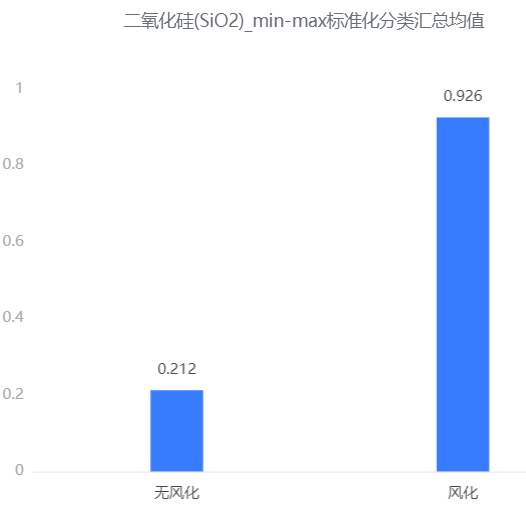
\includegraphics[width=1\textwidth]{Q1-2 (1)}
	\end{minipage}
	\begin{minipage}[b]{0.22\linewidth}
		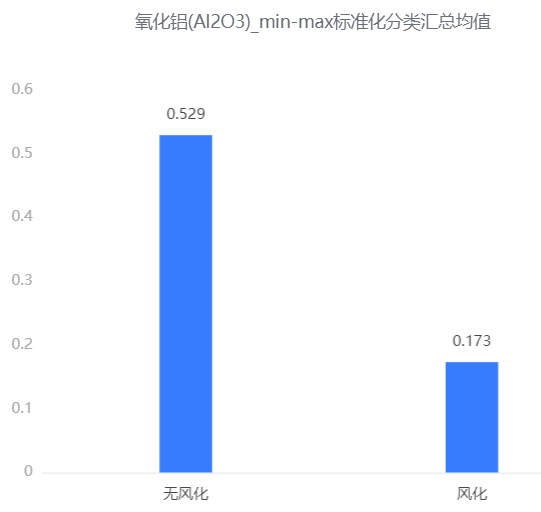
\includegraphics[width=1\textwidth]{Q1-2 (2)}
	\end{minipage}
	\begin{minipage}[b]{0.22\linewidth}
		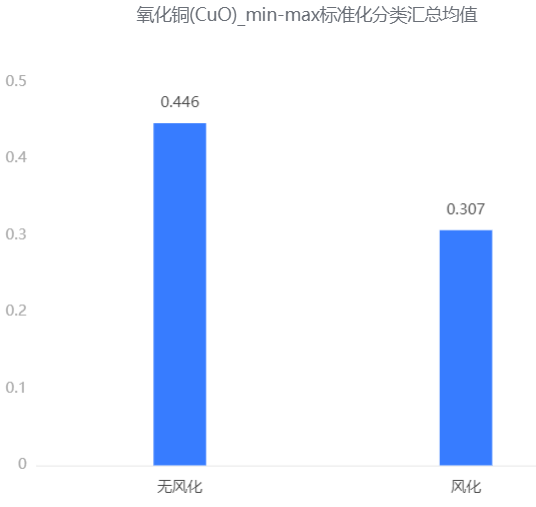
\includegraphics[width=1\textwidth]{Q1-2 (3)}
	\end{minipage}
	\begin{minipage}[b]{0.22\linewidth}
		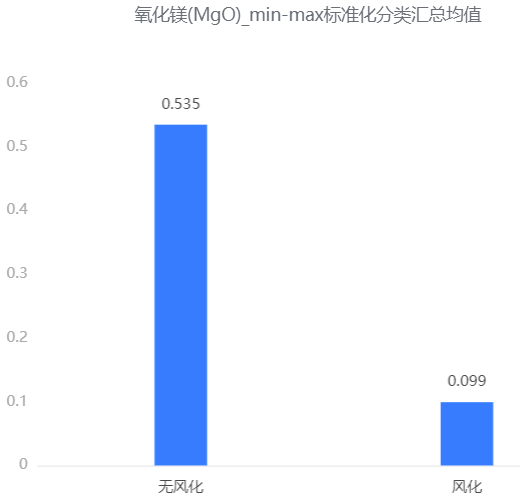
\includegraphics[width=1\textwidth]{Q1-2 (4)}
	\end{minipage}
	\caption{部分成分柱状图显示}
	\label{p-5}
\end{figure}

接下来通过正态性检验对数据进行Shapiro-Wilk(小数据样本,一般样本数5000以下)或者Kolmogorov–Smirnov(大数据样本,一般样本数5000以上)检验,查看其显著性;分析结果中如若不呈现出显著性(p值大于0.05或0.01,严格为0.05,不严格为0.01),说明符合正态分布,反之说明不符合正态分布;

\begin{figure}[h]
	\centering
	\begin{minipage}[b]{0.22\linewidth}
		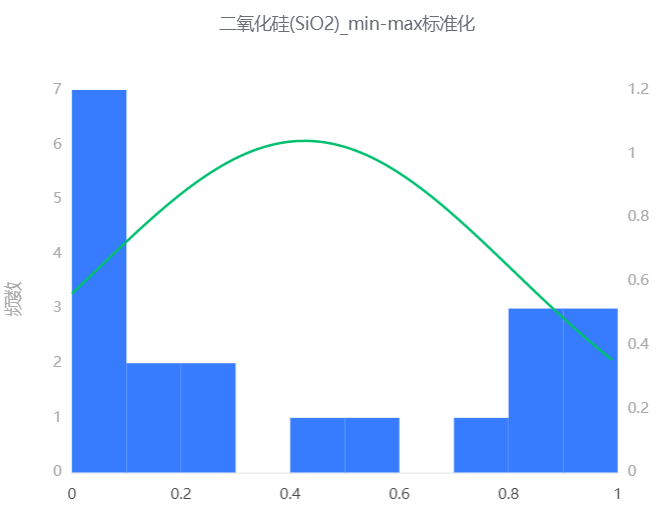
\includegraphics[width=1\textwidth]{Q1-2-1 (1)}
	\end{minipage}
	\begin{minipage}[b]{0.22\linewidth}
		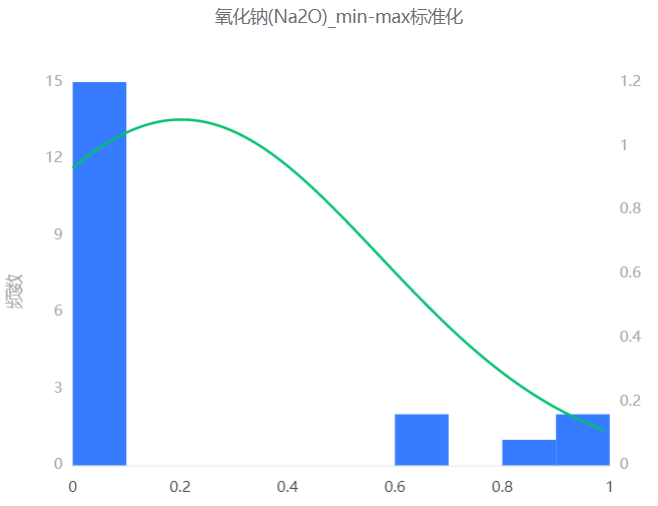
\includegraphics[width=1\textwidth]{Q1-2-1 (2)}
	\end{minipage}
	\begin{minipage}[b]{0.22\linewidth}
		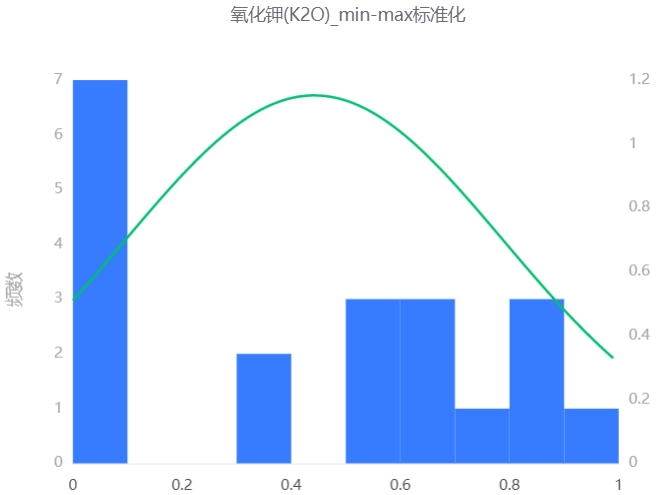
\includegraphics[width=1\textwidth]{Q1-2-1 (3)}
	\end{minipage}
	\begin{minipage}[b]{0.22\linewidth}
		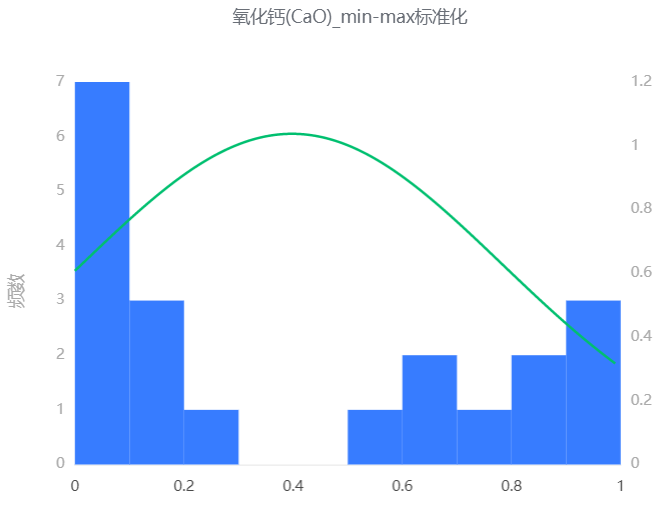
\includegraphics[width=1\textwidth]{Q1-2-1 (4)}
	\end{minipage}
	\caption{部分成分正态性检验直方图显示}
	\label{p-6}
\end{figure}

图\ref{p-6}展示了经过标准化后的数据的正态性检验直方图,正态图基本上呈现出钟型(中间高,两端低),则说明数据虽然不是绝对正态,但是基本可以接受为正态分布。

\subsubsection{建立多元线性回归模型}
在数据预处理中,由于玻璃类型、风化、颜色等指标为定类变量,因此,需要通过独热编码对这些指标进行编码,使其转化为二进制。

多元线性回归(multiple linear regression)是研究一个连续型因变量和多个自变量之间线性关系的统计学分析方法。

1. 模型
多元线性回归分析的模型为
\begin{align}
	\left\{\begin{array}{l}
		y=\beta_0+\beta_1 x_1+\cdots+\beta_m x_m+\varepsilon, \\
		\varepsilon \sim N\left(0, \sigma^2\right),
	\end{array}\right.
\end{align}


式中: $\beta_0, \beta_1, \cdots, \beta_m, \sigma^2$ 都是与 $x_1, x_2, \cdots, x_m$ 无关的末知参数, $\beta_0, \beta_1, \cdots, \beta_m$ 称为回归 系数。

现得到 $n$ 个独立观测数据 $\left[b_i, a_{i 1}, \cdots, a_{i \mathrm{~m}}\right]$, 其中 $b_i$ 为 $y$ 的观察值, $a_{i 1}, \cdots, a_{i m}$ 分别为 $x_1, x_2, \cdots, x_m$ 的观察值, $i=1, \cdots, n, n>m$, 由式 (1)得
\begin{align}
	\left\{\begin{array}{l}
		b_i=\beta_0+\beta_1 a_{i 1}+\cdots+\beta_m a_{i m}+\varepsilon_i, \\
		\varepsilon_i \sim N\left(0, \sigma^2\right), \quad i=1, \cdots, n_{\text {。 }}
	\end{array}\right.
\end{align}
记
\begin{align}
	\begin{gathered}
		\boldsymbol{X}=\left[\begin{array}{cccc}
			1 & a_{11} & \cdots & a_{1 m} \\
			\vdots & \vdots & \ddots & \vdots \\
			1 & a_{n 1} & \cdots & a_{n m}
		\end{array}\right], \quad \boldsymbol{Y}=\left[\begin{array}{c}
			b_1 \\
			\vdots \\
			b_n
		\end{array}\right], \\
		\boldsymbol{\varepsilon}=\left[\varepsilon_1, \cdots, \varepsilon_n\right]^{\mathrm{T}}, \boldsymbol{\beta}=\left[\boldsymbol{\beta}_0, \boldsymbol{\beta}_1, \cdots, \boldsymbol{\beta}_m\right]^{\mathrm{T}},
	\end{gathered}
\end{align}
式 (1)表示为
\begin{align}
	\left\{\begin{array}{l}
		\boldsymbol{Y}=\boldsymbol{X} \boldsymbol{\beta}+\boldsymbol{\varepsilon}, \\
		\boldsymbol{\varepsilon} \sim N\left(0, \sigma^2 \boldsymbol{E}_n\right),
	\end{array}\right.
\end{align}
式中: $\boldsymbol{E}_n$ 为 $n$ 阶单位矩阵。

3. 统计分析

不加证明地给出以下结果:

(1) $\hat{\boldsymbol{\beta}}$ 是 $\boldsymbol{\beta}$ 的线性无偏最小方差估计; $\hat{\boldsymbol{\beta}}$ 的期望等于 $\boldsymbol{\beta}$; 在 $\boldsymbol{\beta}$ 的线性无偏估计中, $\hat{\boldsymbol{\beta}}$ 的 方差最小。

(2) $\hat{\boldsymbol{\beta}}$ 服从正态分布
\begin{align}
	\quad \hat{\boldsymbol{\beta}} \sim N\left(\boldsymbol{\beta}, \sigma^2\left(\boldsymbol{X}^{\top} \boldsymbol{X}\right)^{-1}\right)
\end{align}
记 $\left(\boldsymbol{X}^{\top} \boldsymbol{X}\right)^{-1}=\left(c_{i j}\right)_{n \times n} $。



通过代码求解,可以得出F检验的分析描述,例如:从F检验的结果分析可以得到,显著性P值为0.000***,水平上呈现显著性, 拒绝回归系数为0的原假设, 因此模型基本满足要求。

求得的结果详见附件``风化文物未风化点风化前的化学成分含量.csv''

\subsection{问题二的建模与求解}
需要我们以高钾玻璃和铅钡玻璃两种类型进行进一步分类以及亚类划分,并且针对具体分类模型作出合理性和敏感性分析,我们建立玻璃类型的整体聚类模型,在此基础上根据标准差进行二类划分,问题二建模流程如下图\ref{p-3}所所示:
\begin{figure}[!htbp]
	\centering
	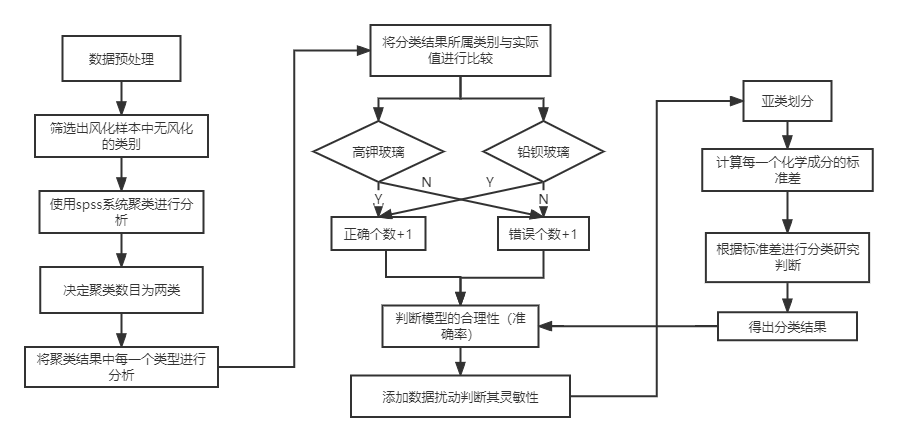
\includegraphics[width=1\textwidth]{流程图2.png}
	\setlength{\abovecaptionskip}{3pt}%caption与表格之间的距离
	\caption{问题二求解流程图}
	\label{p-7}
\end{figure}


\subsubsection{数据预处理}
首先,通过Python代码将附件中的相关数据进行提取,重新生成新文件。其中包含玻璃类型以及所有化学成分。通过查看文件可以看出文件只包含了高钾玻璃和铅钡玻璃两种。通过筛选,分别得出高钾玻璃数据集和铅钡玻璃数据集。

\subsubsection{分析两种玻璃的分类规律}
根据问题一求解得到的不同类型玻璃中风化前后的特征值,通过进行分类汇总,分析两种玻璃的分类规律。
\begin{figure}[!htbp]
	\centering
	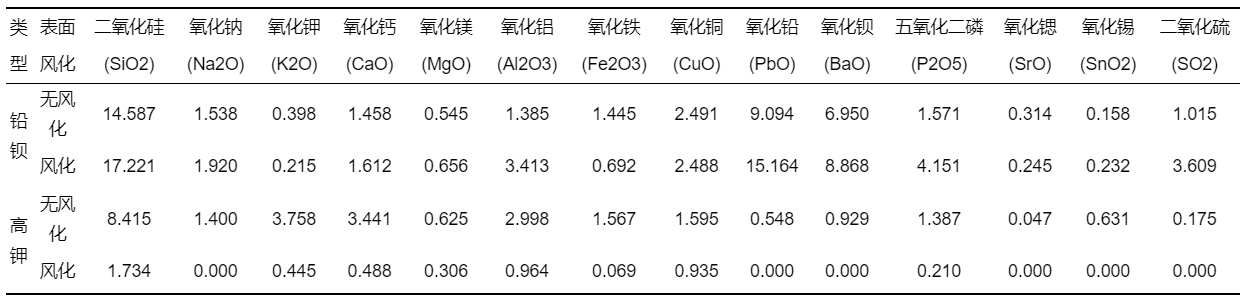
\includegraphics[width=1\textwidth]{Q2-1分类汇总表.png}
	\setlength{\abovecaptionskip}{3pt}%caption与表格之间的距离
	\caption{两种玻璃的分类汇总}
	\label{p-8}
\end{figure}

选取部分化学成分进行柱形图展示,显示效果如图\ref{p-8}
\begin{figure}[h]
	\centering
	\begin{minipage}[b]{0.45\linewidth}
		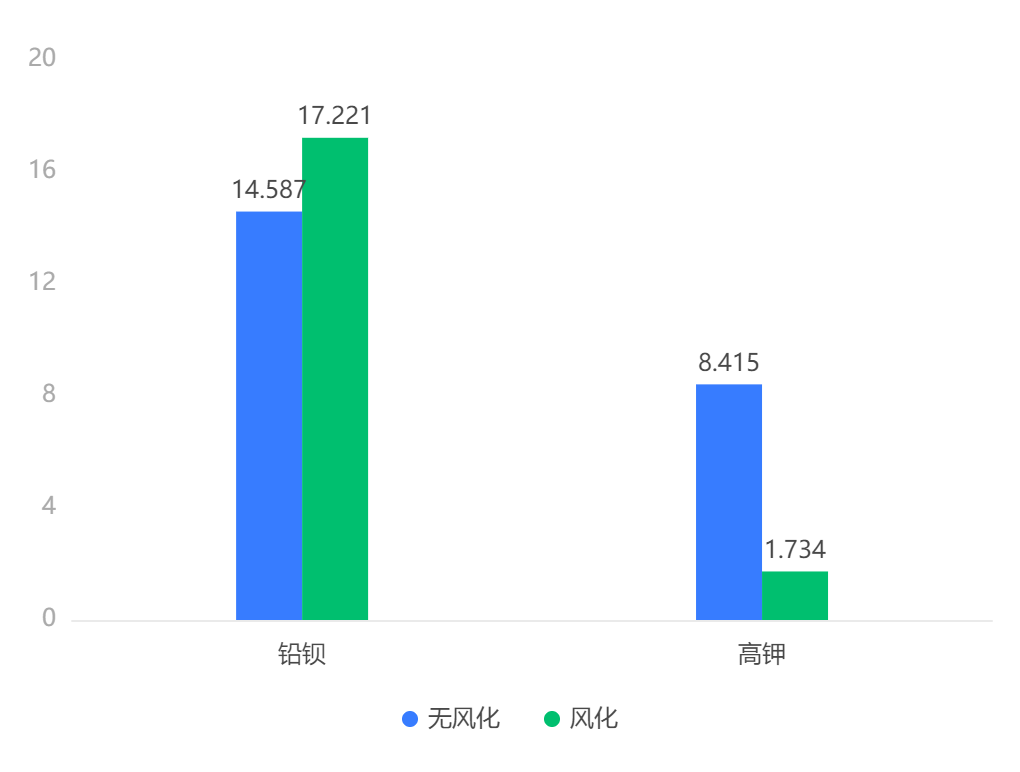
\includegraphics[width=1\textwidth]{Q2-1-1 (1).png}		
	\end{minipage}
	\begin{minipage}[b]{0.45\linewidth}
		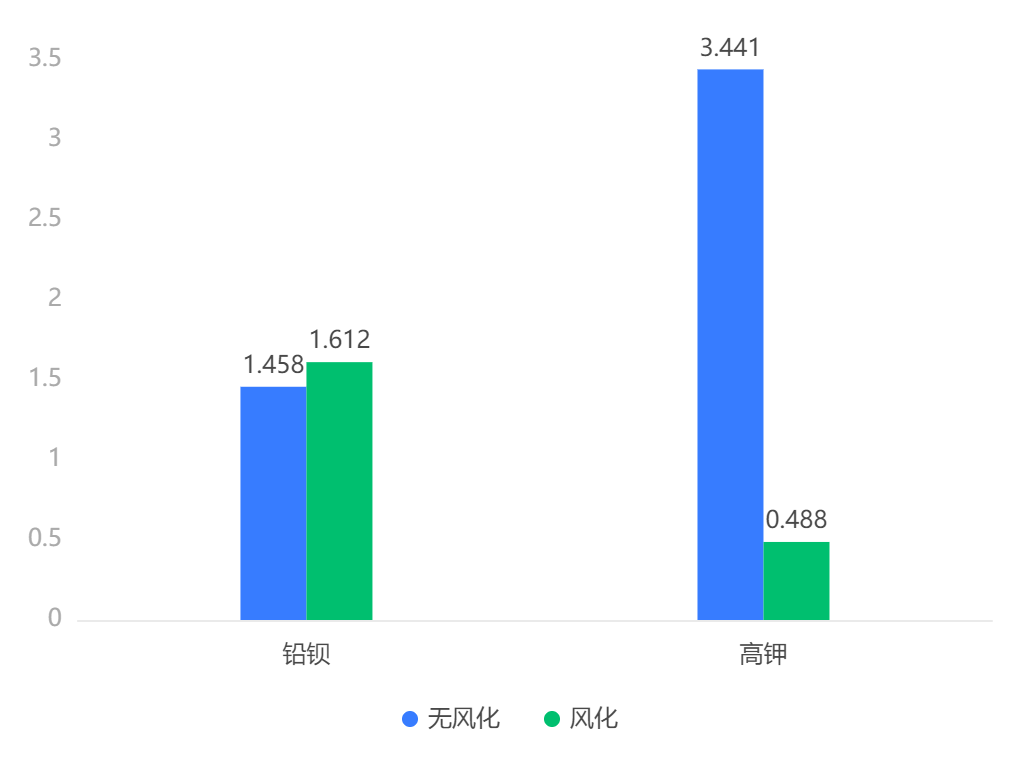
\includegraphics[width=1\textwidth]{Q2-1-1 (2).png}		
	\end{minipage}
	\begin{minipage}[b]{0.45\linewidth}
		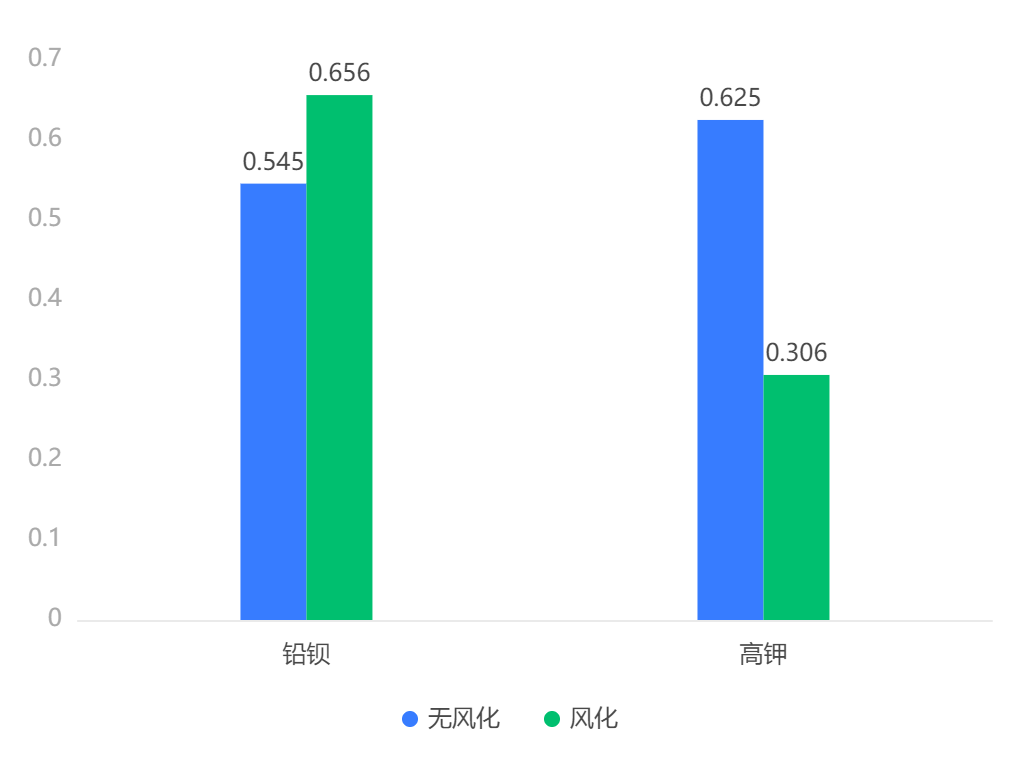
\includegraphics[width=1\textwidth]{Q2-1-1 (3).png}		
	\end{minipage}
	\begin{minipage}[b]{0.45\linewidth}
		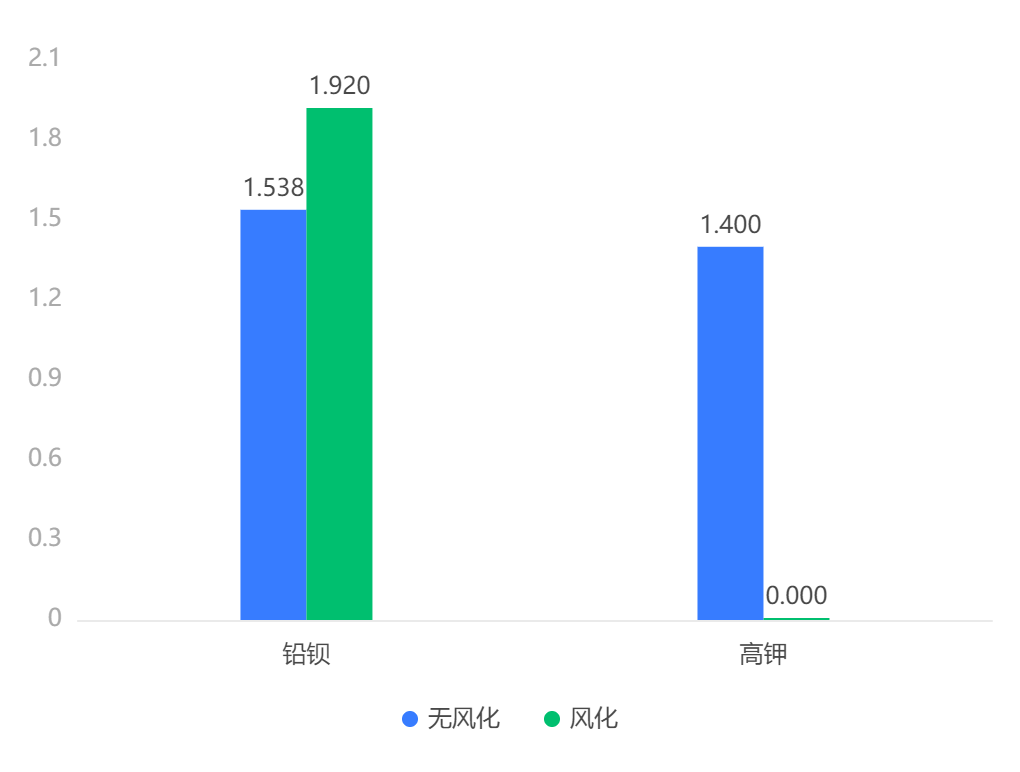
\includegraphics[width=1\textwidth]{Q2-1-1 (4).png}
	\end{minipage}
	\setlength{\abovecaptionskip}{3pt}%caption与表格之间的距离
	\caption{铅钡、高钾玻璃有无风化部分化学成分统计分析}
	\label{p-9}
\end{figure}

通过显示的部分主要化学成分可以看出在铅钡玻璃更加容易风化。

\subsection{聚类划分}
\subsubsection{聚类算法的概念}
聚类算法:一种典型的无监督学习算法,主要用于将相似的样本自动归到一个类别中。

在聚类算法中根据样本之间的相似性,将样本划分到不同的类别中,对于不同的相似度计算方法,会得到不同的聚类结果,常用的相似度计算方法有欧式距离法。

聚类算法是无监督的学习算法,而分类算法属于监督的学习算法。

\subsubsection{k-means聚类步骤}

\begin{enumerate}
	\item 随机设置K个特征空间内的点作为初始的聚类中心
	\item 对于其他每个点计算到K个中心的距离,未知的点选择最近的一个聚类中心点作为标记类别
	\item 接着对着标记的聚类中心之后,重新计算出每个聚类的新中心点(平均值)
	\item 如果计算得出的新中心点与原中心点一样(质心不再移动),那么结束,否则重新进行第二步过程
\end{enumerate}
\begin{figure}[!htbp]
	\centering
	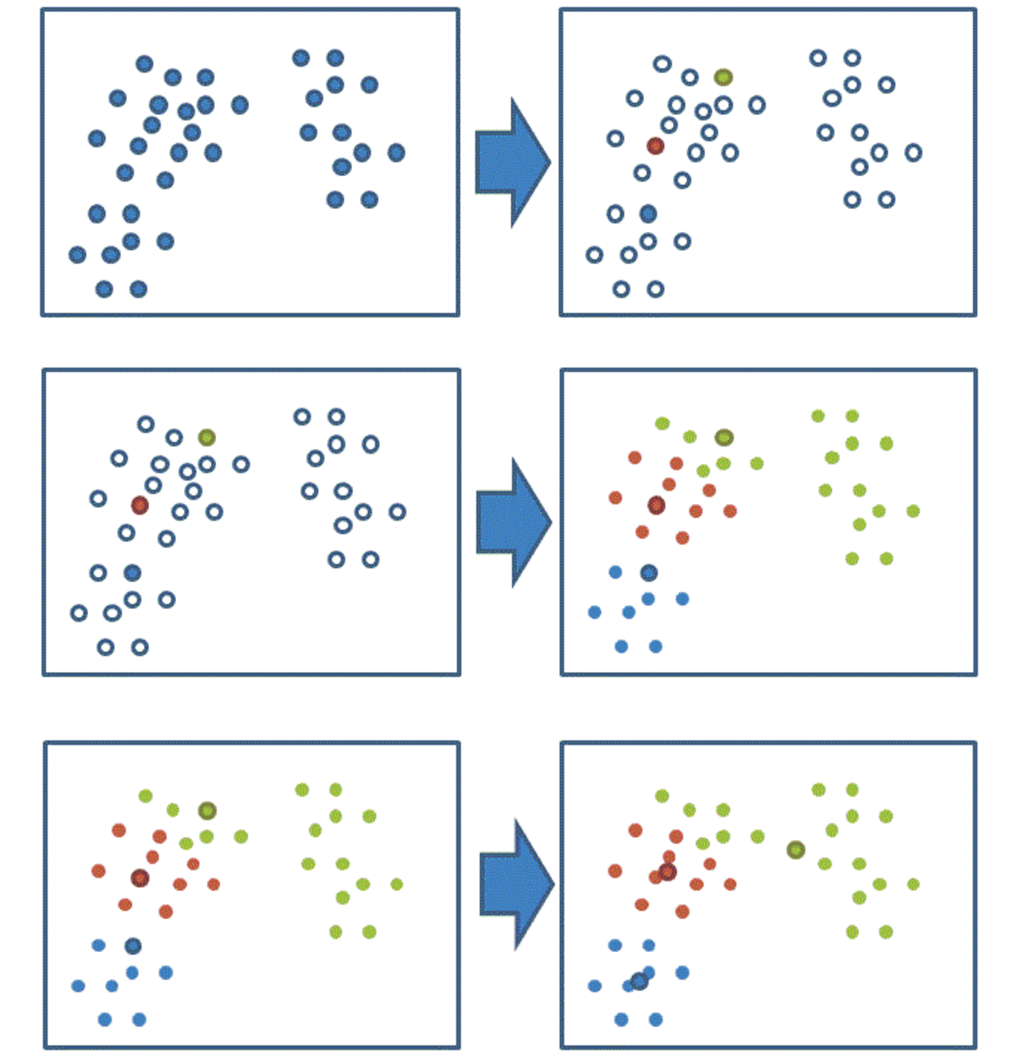
\includegraphics[height=10cm]{K-means过程分析.png}
	\setlength{\abovecaptionskip}{3pt}%caption与表格之间的距离
	\caption{K-means过程分析}
	\label{p-10}
\end{figure}

\subsubsection{``肘''方法-K值确定}
\begin{figure}[!htbp]
	\centering
	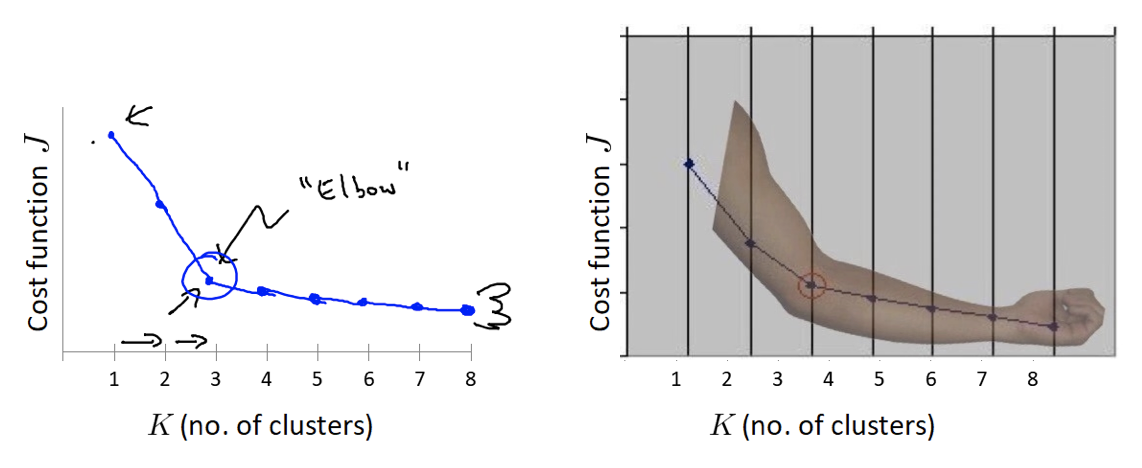
\includegraphics[width=1\textwidth]{elbow_method.png}
	\setlength{\abovecaptionskip}{3pt}%caption与表格之间的距离
	\caption{``肘''方法确定k值}
	\label{p-11}
\end{figure}
\begin{align}
	\sum_{i=0}^n \min _{\mu_j \in C}\left(\left\|x_i-\mu_j\right\|^2\right)
\end{align}
一般情况下会计算K值从2-10的情况,然后得出上述的elbow图,最后选择最优的那个K值。

(1)对于n个点的数据集,迭代计算k from 1 to n,每次聚类完成后计算每个点到其所属的簇中心的距离的平方和;

(2)平方和是会逐渐变小的,直到k==n时平方和为0,因为每个点都是它所在的簇中心本身。

(3)在这个平方和变化过程中,会出现一个拐点也即“肘”点,下降率突然变缓时即认为是最佳的k值。

在决定什么时候停止训练时,肘形判据同样有效,数据通常有更多的噪音,在增加分类无法带来更多回报时,我们停止增加类别。
\begin{figure}[!h]
	\centering
	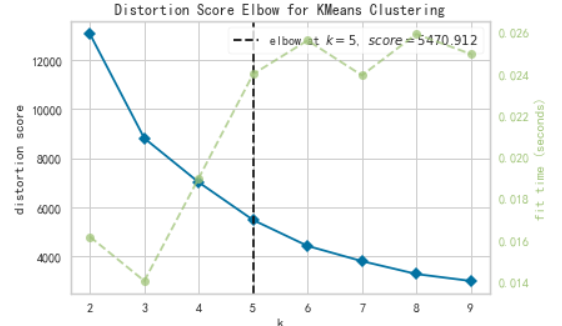
\includegraphics[width=0.4\textheight]{亚分类}
	\setlength{\abovecaptionskip}{3pt}%caption与表格之间的距离
	\caption{Kmeans聚类分析}
	\label{p-12}
\end{figure}
由图\ref{p-12}可以看出聚类分析中,k值为3或者4时能够取得比较好的效果。

\subsection{问题三的建模与求解}
\subsubsection{数据集特征生成}
首先需要需要从附件表单二中提取出类型、表面风化以及化学成分等特征数据,然后需要对表面风化定类特征进行独热编码,从而生成两个新特征。

\subsubsection{模型建立}
逻辑回归(Logistic Regression)模型是一种对数线性模型,模型解释性强且原理易理解,它是统计学中的经典分类方法。

逻辑回归模型的分布函数和密度函数分别为:
\begin{align}
	F(x)=P(X\le x) = \frac{1}{1+exp(-(x-\mu)/\gamma)}
\end{align}

\begin{align}
	f(x)=F'(x) = \frac{exp(-(x-\mu)/\gamma)}{\gamma(1+exp(-(x-\mu)/\gamma))^2}
\end{align}

其中,$\mu$为位置参数,$\gamma>0$为形状参数。逻辑回归模型的分布函数是一条S型曲线,参数$\gamma$的值越小,曲线在中心处位置增长的就越快。

逻辑回归模型可以做二分类和多分类,本文主要介绍逻辑回归的二分类算法。逻辑回归模型二分类算法的条件概率分布如下:
\begin{align}
	P(Y=1|x)=\frac{exp(\theta x + b)}{1 + exp(\theta x + b)}
\end{align}
\begin{align}
	P(Y=0|x)=\frac{1}{1 + exp(\theta x + b)}
\end{align}


其中,$x$为特征变量,$Y\in {0,1}$为目标变量,$\theta$为权值向量,$b$为偏置。由式(6)和式(7)可得
\begin{align}
	log\frac{P(Y=1|x)}{1-P(Y=0|x)}=\theta x + b
\end{align}

逻辑回归模型训练时,对于给定的训练数据集D,设$P(Y=1|x)=\varphi(x),P(Y=1|x)=1-\varphi(x)$,似然函数为
\begin{align}
	\prod^N_{i=1}[\varphi(X_i)]^{y_i}[\varphi(X_i)]^{1-y_i}
\end{align}

对数似然函数为
\begin{align}
	L(\theta)&=\sum^N_{i=1}[y_ilog\varphi(x_i) + (1-y_i)log(1-\varphi(x_i))]\\
	&=\sum^N_{i=1}[y_ilog\frac{\varphi(x_i)}{1-\varphi(x_i)}+log(1-\varphi(x_i))]\\
	&=\sum^N_{i=1}[y_i(\theta x_i)-log(1+e^{\theta x_i})]
\end{align}
对$L(\theta)$求极大值,得到$\theta$的估计值$\hat{\theta}$。
\begin{align}
	h(w)=w_1 x_1+w_2 x_2+w_3 x_3 \ldots+b
\end{align}

激活函数 
\begin{itemize}
	\item sigmoid函数
	\begin{align}
		g\left(w^T, x\right)=\frac{1}{1+e^{-h(w)}}=\frac{1}{1+e^{-w^T x}}
	\end{align}
	\item 判断标准
	\begin{itemize}
		\item 回归的结果输入到sigmoid函数当中
		\item 输出结果:[0, 1]区间中的一个概率值,默认为0.5为阈值
		\begin{figure}[!h]
			\centering
			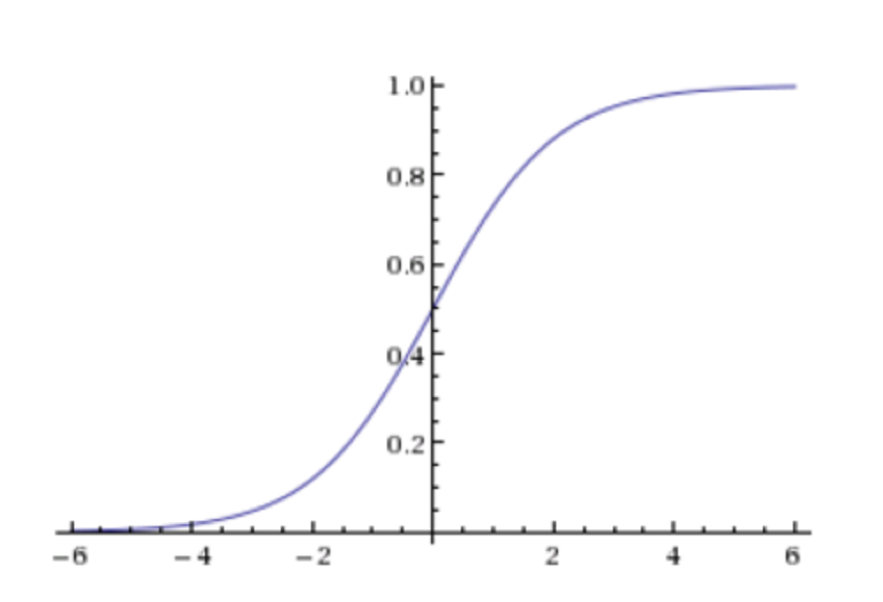
\includegraphics[width=0.4\textheight]{sigmoid图像.png}
			\setlength{\abovecaptionskip}{3pt}%caption与表格之间的距离
			\caption{sigmoid图像}
			\label{p-13}
		\end{figure}
	\end{itemize}
\end{itemize}

逻辑回归最终的分类是通过属于某个类别的概率值来判断是否属于某个类别,并且这个类别默认标记为1(正例),另外的一个类别会标记为0(反例)。\textsuperscript{\cite{b3}}

下图中,设置阈值为0.6
\begin{figure}[!h]
	\centering
	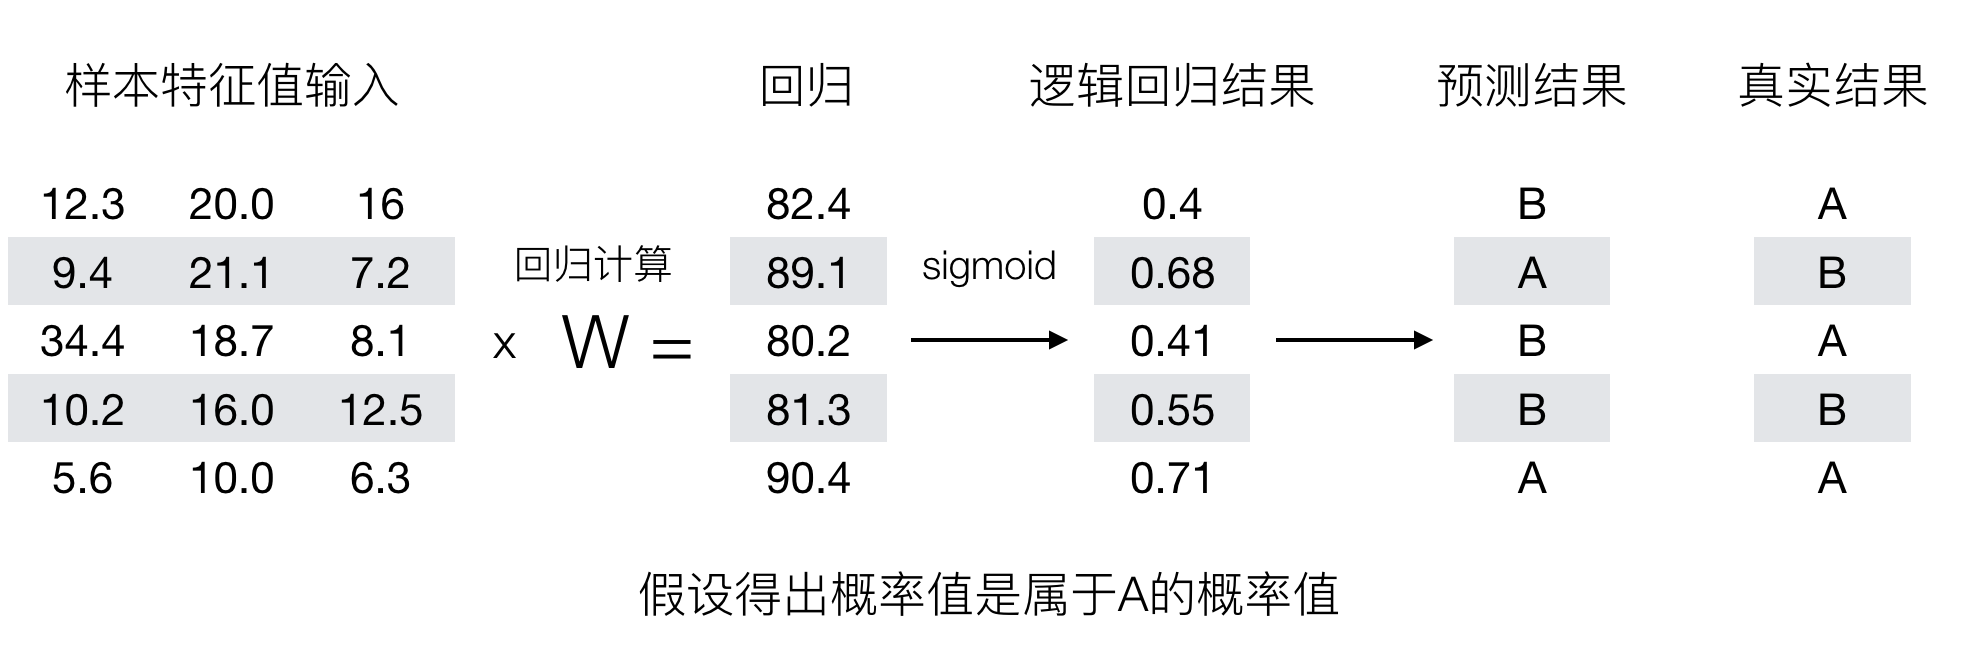
\includegraphics[width=0.6\textheight]{逻辑回归运算过程.png}
	\setlength{\abovecaptionskip}{3pt}%caption与表格之间的距离
	\caption{逻辑回归运算过程}
	\label{p-14}
\end{figure}

\subsubsection{数据集划分}
经过数据集划分,将原始数据划分为训练数据和测试数据,建立模型之后,通过对训练集进行训练,得到基础模型,然后通过测试集进行模型预测。

\subsubsection{模型评估}
\begin{table}[h]
	\centering
	\setlength{\abovecaptionskip}{3pt}%caption与表格之间的距离
	\caption{逻辑回归模型分析}
	\vspace{1pt}
	\label{t-5}
	\resizebox{\textwidth}{!}{
		\begin{tabular}{ccccc}
			\toprule[1.5pt]
			\makebox[0.18\textwidth][c]{逻辑回归} & \makebox[0.18\textwidth][c]{precision} 
			& \makebox[0.18\textwidth][c]{recall} & \makebox[0.18\textwidth][c]{precsion}
			& \makebox[0.18\textwidth][c]{F1-Socre} \\ 
			\midrule
			训练集&	1&	1&	1&	1\\
			交叉验证集&	0.75&	0.75&	0.78&	0.747\\
			测试集	&0.905	&0.905&	0.905&	0.905\\
			\bottomrule[1.5pt]
	\end{tabular}}
\end{table}

表\ref{t-5}显示了对逻辑回归模型进行预测的结果,总体上模型效果优良,预测效果较好。

\subsubsection{预测模型评价指标}
模型性能评价指标是选择模型优劣的重要参考,评价指标主要有准确率、混淆矩阵、F1分数以及ROC曲线。

\begin{itemize}
	\item 准确率
	
	评价分类器性能的指标一般是分类准确率( accuracy),是用来表示模型分类正确总度量。它的计算方式为测试集样本数据中模型预测结果预测正确数量之和比上测试集样本总量,即:
	\begin{align}
		\text{准确率}=\frac{\sum^n_{i=1}\text{预测结果类别为}i\text{且实际类别也为}i\text{的样本数量}}{\text{总样本量}}
	\end{align}
	
	精度能够直观的判断分类模型的分类准确程度,但在判断之前需要确认样本数据是否存在样本过采样、欠采样问题。比如说数据集样本总量为N,有i个类别,其中某一类别Ⅰ占数据总量的90\%,如果模型预测结果类别全为l,模型的预测的准确率则为90\%。
	
	\item F1-Score
	
	从计算公式可以看出精确率与召回率之间有着某种联系,精确率高时召回率相对会低,因此延伸出精确率与召回率的调和均值F1,即
	
	\begin{align}
		\frac{2}{F1}=\frac{1}{P}+\frac{1}{R}
		F1=2\frac{R * P}{R + P} = \frac{2TP}{2TP + FP + FN}
	\end{align}
	精确率Р和召回率R他们的值都高时,F1值也高。
	
	\item  交叉验证
	
	交叉验证是验证分类器性能的一种统计分析方法,它的工作原理是将原始数据集分为训练集和验证集,用训练集进行训练模型,然后使用验证集对模型进行验证,以此作为评价分类器性能的指标。
	
	Hold-Out Method方法是将数据集随机分为训练集和验证集两组,一组用来训练模型,一组用来验证模型的性能,此方法因没有达到交叉验证的效果并不常用。
	
	Double Cross Validation思想是先将数据集分为大小相等的两个子集,一个子集作为训练集一个作为测试集训练分类器,然后将训练集与测试集对换在此训练模型,两次训练集的辨识度作为输出的结果,其中不足之处在于训练集样本的分布不足以代表数据集总体样本分布。\textsuperscript{\cite{b8}}
	
	K-fold Cross Validation思想是将数据集分成K组,在K组中每个子集做一次验证集,余下的K-1组用来训练分类器,得到K个训练模型。
	
\end{itemize}

